% !TeX spellcheck = <none>
%==============================================================================
% Sjabloon onderzoeksvoorstel bachelorproef
%==============================================================================
% Gebaseerd op LaTeX-sjabloon ‘Stylish Article’ (zie voorstel.cls)
% Auteur: Jens Buysse, Bert Van Vreckem

% TODO: Compileren document:
% 1) Vervang ‘naam_voornaam’ in de bestandsnaam door je eigen naam, bv.
%    buysse_jens_voorstel.tex
% 2) latexmk -pdf naam_voornaam_voorstel.tex
% 3) biber naam_voornaam_voorstel
% 4) latexmk -pdf naam_voornaam_voorstel.tex (1 keer)

\documentclass[fleqn,10pt]{voorstel}
\usepackage[dutch]{babel}
\usepackage{graphicx}

%------------------------------------------------------------------------------
% Metadata over het artikel
%------------------------------------------------------------------------------

\JournalInfo{HoGent Bedrijf en Organisatie} % Journal information
\Archive{Bachelorproef 2018 - 2019} % Additional notes (e.g. copyright, DOI, review/research article)

%---------- Titel & auteur ----------------------------------------------------

\PaperTitle{Het gebruik van Computer Vision API's voor de beschrijving van cultureel-erfgoedcollecties}
\PaperType{Onderzoeksvoorstel Bachelorproef} % Type document

\Authors{Nastasia Vanderperren\textsuperscript{1}} % Authors
\affiliation{\textbf{Contact:}
  \textsuperscript{1} \href{mailto:jens.buysse@hogent.be}{nastasia.vanderperren.v8632@student.hogent.be}}

%---------- Abstract ----------------------------------------------------------

  \Abstract{Om de registratieachterstand bij collectiebeherende instellingen in Vlaanderen weg te werken, dient een inhaalbeweging gemaakt te worden. We stellen in dit onderzoek voor om hiervoor Computer Vision API's in te schakelen. Het onderzoek wil zich focussen op het analyseren van de metadatavelden die geschikt zijn voor Computer Vision, de voorwaarden die nodig zijn om tot een succesvol resultaat te komen en een vergelijking te maken tussen de bestaande diensten. We willen weten of deze software in de toekomst gebruikt kan worden om het werk van de registratoren te verlichten en achterstanden weg te werken.}

%---------- Onderzoeksdomein en sleutelwoorden --------------------------------
%
% Het eerste sleutelwoord beschrijft het onderzoeksdomein. Je kan kiezen uit
% deze lijst:
%
% - Mobiele applicatieontwikkeling
% - Webapplicatieontwikkeling
% - Applicatieontwikkeling (andere)
% - Systeem- en netwerkbeheer
% - Mainframe
% - E-business
% - Databanken en big data
% - Machine learning en kunstmatige intelligentie
% - Andere (specifieer)
%
% De andere sleutelwoorden zijn vrij te kiezen

\Keywords{Onderzoeksdomein. Machine learning en kunstmatige intelligentie --- Computer Vision --- Digital humanities} % Keywords
\newcommand{\keywordname}{Sleutelwoorden} % Defines the keywords heading name

%---------- Titel, inhoud -----------------------------------------------------
\begin{document}

\flushbottom % Makes all text pages the same height
\maketitle % Print the title and abstract box
\tableofcontents % Print the contents section
\thispagestyle{empty} % Removes page numbering from the first page

%------------------------------------------------------------------------------
% Hoofdtekst
%------------------------------------------------------------------------------

%---------- Inleiding ---------------------------------------------------------

\section{Introductie} % The \section*{} command stops section numbering
\label{sec:introductie}

De Vlaamse Overheid investeert in het Vlaamse cultureel erfgoed door collectiebeherende instellingen te ondersteunen en kwaliteitslabels uit te reiken. In ruil voor die steun verwacht de Vlaamse Overheid dat die instellingen een aantal taken uitvoeren, waaronder het registreren, inventariseren en metadateren van cultureel-erfgoedobjecten op een gestandaardiseerde manier, het onderzoeken (en faciliteren van onderzoek) en het presenteren van de collectie.~\autocites{AKE2014}{Gatz2016}

De collectiebeherende instellingen lijden aan een historische achterstand m.b.t. de registratie van de eigen collectie~\autocite{Gatz2016}. In 2018 werd daarom een nieuwe subsidielijn opgestart om de digitale collectieregistratie weg te werken. Deze subsidielijn werd opgestart vanuit de vaststelling dat de competenties en strategieën ontbreken om een inhaalbeweging te realiseren~\autocite{JeugdMediaC2018a}.

In de bachelorproef willen we onderzoeken in welke mate Computer Vision API's (vanaf nu afgekort als CVA), zoals Google Cloud Vision\footnote{\url{https://cloud.google.com/vision/}} of Microsoft Computer Vision API\footnote{\url{https://azure.microsoft.com/nl-nl/services/cognitive-services/computer-vision/}}, ingezet kunnen worden om dit registratieproces te versnellen en als strategie gebruikt kunnen worden om een inhaalbeweging te realiseren. Momenteel moet ieder erfgoedobject geregistreerd worden door een domeinexpert. Dit is tijdrovend werk. Met behulp van artificiële intelligentie (AI) kan dit proces ten dele geautomatiseerd worden. Dit geeft de collectieregistrator de mogelijkheid om zich met minder basaal werk bezig te houden, zoals het verrijken van de data of het klaarmaken van de data om ze als open (linked) data vrij te geven, nog een beleidslijn waar de Vlaamse Overheid op wil inzetten~\autocite{JeugdMediaC2018}. 

Figuren 1 t.e.m. 4 geven een voorbeeld van de registratieachterstand in musea. De cijfers zijn afkomstig van de VKC Datahub Dashboard.\footnote{\url{https://dashboard.vlaamsekunstcollectie.be}} Dit dashboard analyseert de collectieregistratie van de Vlaamse musea voor Schone (en in de toekomst ook Hedendaagse) Kunsten die aangesloten zijn bij de VlaamseKunstCollectie (VKC)\footnote{\url{http://vlaamsekunstcollectie.be/}}. Het is bedoeld om de museale medewerker inzicht te geven in de staat van de collectiemetadata van zijn museum in functie van digitale bruikbaarheid. Ze meten onder meer hoeveel records ingevuld zijn volgens de minimale en basisregistratie.\footnote{De CIDOC-richtlijnen, ook wel de minimale registratie genoemd, gelden als de absolute minimum voor het beschrijven van objecten in museale collecties. Ook de basisregistratie is een minimumrichtlijn die afkomstig is van CIDOC. Voor meer info, zie \href{http://network.icom.museum/fileadmin/user_upload/minisites/cidoc/DocStandards/CIDOC_Fact_Sheet_No_1.pdf}{CIDOC Fact Sheet No. 1: Registration step by step(1993)} en \href{https://www.projectcest.be/wiki/Richtlijn:Objecten_registreren}{CEST-Richtlijn: Objecten registreren}} Dit zijn cijfers van de grooste kunstmusea van Vlaanderen. 

\begin{figure}[h]
	\caption{Het overzicht van de velden van de minimale registratie en het aantal keer dat ze aanwezig zijn in de collectiedata van MSK Gent}
	\centering
	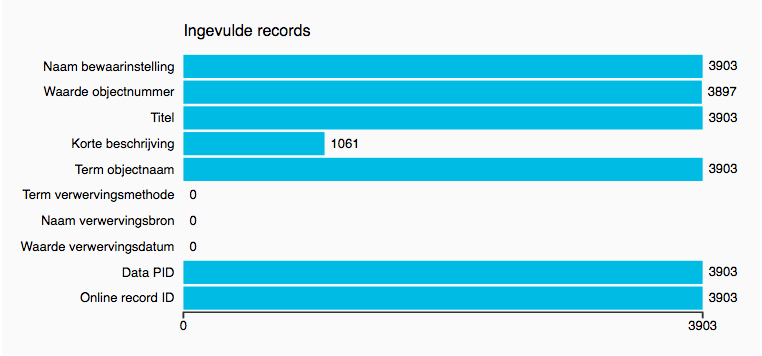
\includegraphics[width=\linewidth]{pictures/VKC_velden_minimale}
\end{figure}

\begin{figure}[h]
	\caption{Het aantal volldig ingevulde records van MSK Gent volgens de minimale registratie}
	\centering
	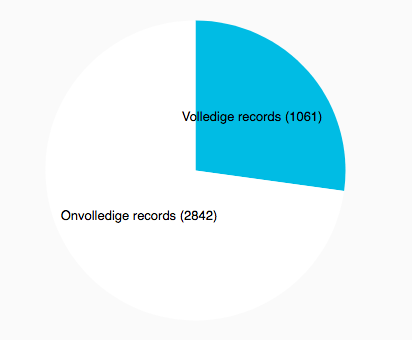
\includegraphics[width=\linewidth]{pictures/VKC_aantal_minimale}
\end{figure}

\begin{figure}[h]
	\caption{Het overzicht van de velden van de basisregistratie en het aantal keer dat ze aanwezig zijn in de collectiedata van MSK Gent}
	\centering
	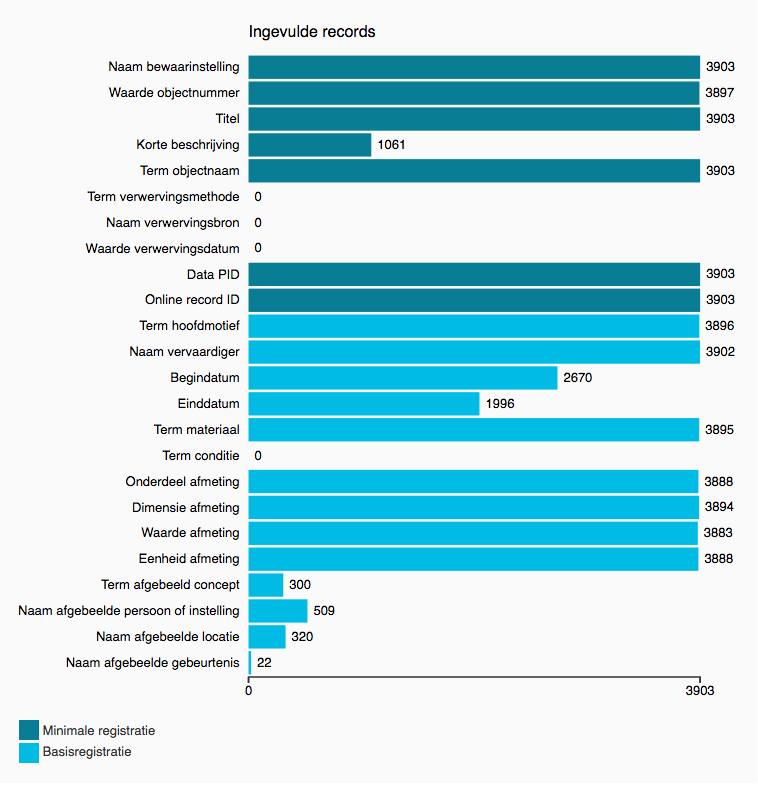
\includegraphics[width=\linewidth]{pictures/VKC_velden_basis}
\end{figure}

\begin{figure}[h]
	\caption{Het aantal volldig ingevulde records van MSK Gent volgens de basisregistratie}
	\centering
	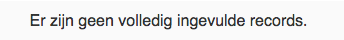
\includegraphics[width=\linewidth]{pictures/VKC_aantal_basis}
\end{figure}


Uit deze cijfers blijkt dat vooral formele en administratieve gegevens geregistreerd worden; inhoudelijke informatie, zoals afgebeelde persoon of afgebeeld concept, die interessant is voor ontsluiting en onderzoek, ontbreekt hoofdzakelijk.

In het verleden werd reeds (theoretisch) onderzoek verricht naar het gebruik van Computer Vision voor cultureel erfgoed en kunst.\footnote{Zie infra, in het deel \emph{Stand van zaken}.} De resultaten van dit onderzoek waren veelbelovend. Nieuwe ontwikkelingen zorgen ervoor dat Computer Vision steeds meer accuraat wordt en steeds eenvoudiger in gebruik, waardoor het meer en meer een instrument wordt waarmee ook developers aan de slag kunnen~\autocite{Hindle2017}.


%---------- Stand van zaken ---------------------------------------------------

\section{Stand van zaken}
\label{sec:state-of-the-art}

\subsection{Computer Vision en (cultureel) erfgoed}
Een aantal instellingen maken al gebruik van Computer Vision voor de ontsluiting van hun collectie:
\begin{itemize}
	\item \textbf{The Museum of Modern Art (MoMA)}\footnote{\url{https://www.moma.org/}} gebruikte diensten van Google via \emph{Google Arts \& Culture Lab} om aan de historische foto's van afgelopen tentoonstellingen in MOMA foto's uit de kunstcollectie te koppelen. Het algoritme analyseerde hiervoor alle foto's van tentoonstellingszichten. Als het een kunstwerk op de foto's kon herkennen, dan werd er een koppeling gelegd met de afbeelding van dit kunstwerk in de collectie van MOMA.\footnote{Bekijk een voorbeeld over \href{https://www.moma.org/calendar/exhibitions/1767/installation_images/10473}{een tentoonstelling over C\`{e}zanne, Gaugain, Seurat en Van Gogh uit 1929}} MOMA stelde hierbij vast dat het logaritme vooral goed scoort op het vlak van tweedimensionele, statische afbeeldingen (bv. een afbeelding van een kunstwerk), maar dat het minder goede resultaten geeft met afbeeldingen van 3D-objecten (bv. een standbeeld) of bewegend beeld~\autocite{MOMA2018?}.
	
	\item Het \textbf{Smithsonian}\footnote{\url{https://www.smithsonianmag.com/}} gebruikt AI-technologie om stalen van planten te classificeren. Het Smithsonian is gestart met het systematisch digitaliseren van de collectie voor wetenschappers en in functie van online ontsluiting. De AI-technologie slaagde erin om via deze afbeeldingen twee gelijkaardige planten te onderscheiden met een succesgraad van meer dan 90\%~\autocite{Smith2017}.
	
	\item Het \textbf{Nasjonalmuseet}\footnote{\url{http://www.nasjonalmuseet.no/en/}} was het onderwerp van het \emph{Principal Components} onderzoek. Hierbij werd met het deep learning framework Caffe\footnote{Voor meer info, zie: \url{http://caffe.berkeleyvision.org/}} gezocht naar compositionele gelijkenissen tussen kunstwerken en werden ze geclassifieerd op basis van de Iconclass-termen\footnote{Iconclass is een gespecialiseerd kunsthistorisch classiciatiesysteem, \url{https://nl.wikipedia.org/wiki/Iconclass}}. Dit resulteerde in een vernieuwende publiekstoegang tot de collectie waarbij de kunstwerken op basis van gelijkenissen gevisualiseerd werden. Hoe meer gelijkenissen, hoe dichter de kunstwerken bij elkaar staan.\footnote{\href{http://vy.nasjonalmuseet.no/?collection=painting_subject}{Bekijk bijvoorbeeld schilderijen op basis van hun motief}.} \autocites{Nasjonalmuseet2017?}{Westvang2017?}
\end{itemize}

\subsection{Theoretisch onderzoek}
Daarnaast is er eerder theoretisch onderzoek gedaan naar het gebruik van Computer Vision binnen een erfgoedcontext. In onderstaande lijst worden de onderzoeken vermeldt die zich focussen op museumcollecties:
\begin{itemize}
	\item \textbf{Using Machine Learning for Identification of Art Paintings (2013)}: In dit onderzoek werd machine learning gebruikt voor het classificeren van kunstwerken van zeven kunstenaars: C\'{e}zanne, Dali, D\"{u}rer, Monet, Picasso, Rembrandt en Van Gogh. Per kunstenaar werden er tweehonderd kunstwerken gezocht. In 87,13\% van de gevallen was de computer correct. De onderzoekers vermoedden dat dit resultaat nog beter kan zijn als de training set groter is.~\autocite{Blessings2013}
	
	\item \textbf{The Rijksmuseum Challenge: Museum-Centered Visual Recognition (2014)}: Beelden die publiek beschikbaar zijn via de API van Het Rijksmuseum\footnote{\url{https://www.rijksmuseum.nl/en/api}} werd gebruikt voor het oplossen van vier challenges: 
	\begin{itemize}
		\item voorspel de kunstenaar van het afgebeelde object;
		\item voorspel het materiaal dat gebruikt werd voor het afgebeelde object;
		\item voorspel het jaar waarin het object gemaakt werd;
		\item voorspel het soort object (schilderij, tekening, standbeeld...) dat afgebeeld wordt.
	\end{itemize}
	Het ging om objecten die afkomstig waren van de oudheid tot de late 19e eeuw en om een veelheid aan objecten: schilderijen, foto's, keramiek, meubels, etc. Ook in dit onderzoek waren de resultaten veelbelovend.~\autocite{Mensink2014}
	
	\item \textbf{INSIGHT (2017-2020)}: Hier wil men onderzoeken hoe AI kan gebruikt worden om collecties uit de cultureel-erfgoedsector van beschrijvende metadata te voorzien. De collecties van de Koninklijke Musea voor Schone Kunsten van België en de Koninklijke Musea voor Kunst \& Geschiedenis worden als testcase gebruikt. De focus ligt op het vrijgeven van die data als open datasets.~\autocite{UniAntwerpen2017?} Uit de paper \emph{Deep Transfer Learning for Art Classification Problems} van \textcite{Sabatelli2018} kwamen veelbelovende resultaten naar boven voor het voorspellen van materiaal, objecttype en kunstenaar.
	
	\item \textbf{Automated Image Analysis with IIIF (2017)}: Dit onderzoek is eerder praktisch gericht en werd uitgevoerd buiten de academische wereld. Het werd uitgevoerd door CogApp, een bedrijf dat software ontwikkelt voor online archieven en musea.\footnote{\url{https://www.cogapp.com/about/}} Zij hebben verschillende testen gedaan met machine learning. Het meest interessant voor dit voorstel is het onderzoek waarbij drie Computer Vision API's (Google Cloud Vision, Microsoft Computer Vision en Clarifai\footnote{\url{https://www.clarifai.com/}}) getest werden om beelden te voorzien van extra tags om de doorzoekbaarheid te verbeteren. Naast de grappige resultaten~\autocite{Roddis2018}, leidde dit tot goede resultaten waarmee de beeldencollectie op een interessante manier doorzocht kan worden: Je kan er een selectie van beelden verkrijgen door te filteren op verschillende tags, bv. \emph{ik wil een kunstwerk uit de Renaissance van iemand met een snor en een cape}.\footnote{Probeer het zelf op: \url{http://labs.cogapp.com/iiif-ml/}} De onderzoekers concludeerden dat de CVA accurate beschrijvingen geven en dat Computer Vision steeds eenvoudiger in gebruik wordt. De foutieve beschrijvingen, zoals in Figuur 6, komen vermoedelijk doordat CVA getraind worden met hedendaagse beelden gemaakt met een smartphone of computer.~\autocite{Hindle2017}
	
	\begin{figure}[h]
		\caption{Een vrouw wordt door  Microsoft Computer Vision geïdentificeerd als een teddybeer~\autocite{Roddis2018}.}
		\centering
		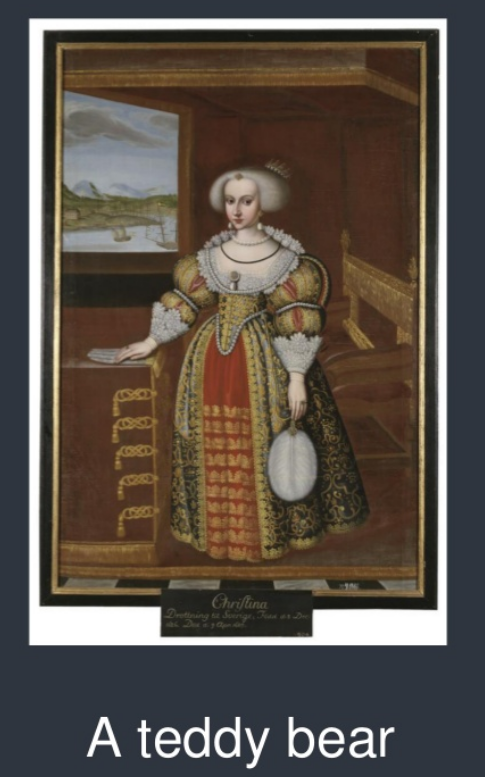
\includegraphics[width=\linewidth]{pictures/roddis_grappig_1}
	\end{figure}

	\begin{figure}[h]
		\caption{Vrouw en man met boek worden door Microsoft Computer Vision ge\"identificeerd als man en vrouw die een selfie nemen~\autocite{Roddis2018}.}
		\centering
		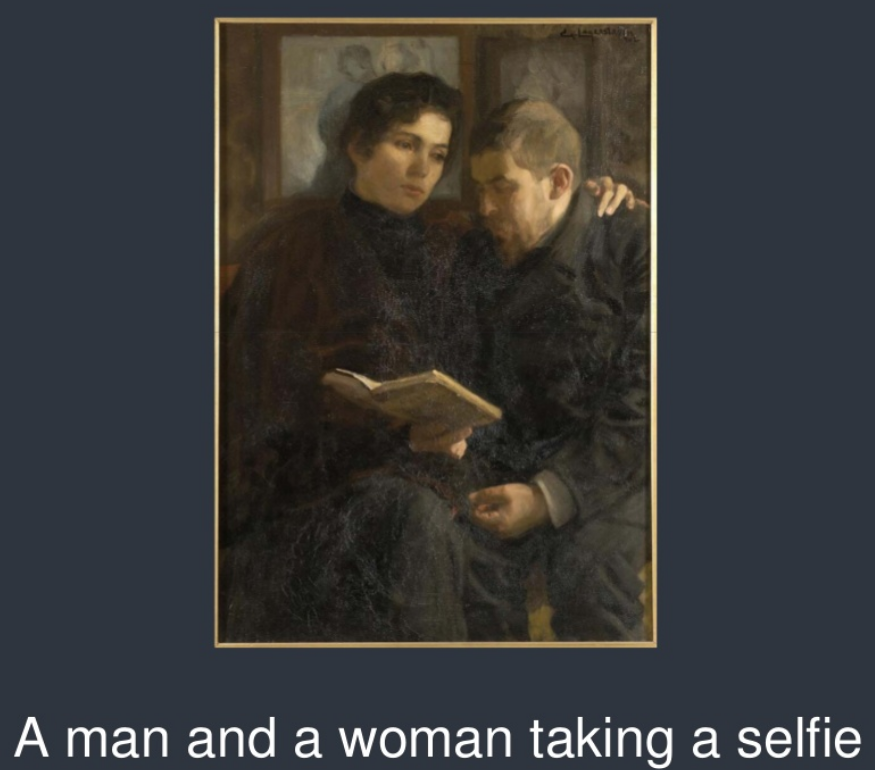
\includegraphics[width=\linewidth]{pictures/roddis_grappig_2}
	\end{figure}

\end{itemize}

\subsection{Computer Vision API's}
Tot slot lichten we kort CVA toe. CVA, ook wel image/visual recognition API's genoemd, zijn API's die afbeeldingen automatisch kunnen taggen, organiseren en zoeken via machine learning. Het biedt de mogelijkheid om machine learning toe te passen zonder dat je hier zelf een expert in moet zijn. Je kan er zelf modellen mee creëren om de API's te trainen naar je eigen behoefte. Zo leerde Matt Fraser Google Cloud Vision verschillende spinnen te herkennen door de dienst te trainen met honderd afbeeldingen per spin~\autocite{Fraser2018}.  De bekendste diensten zijn Clarifai, IBM Visual Recognition\footnote{\url{https://www.ibm.com/watson/services/visual-recognition/}}, Microsoft Computer Vision en Google Cloud Vision.  De diensten zijn zo toegankelijk dat iedere ontwikkelaar zonder machine learning kennis modellen kan bouwen, maar dat ook, volgens TechCrunch, iedereen zonder programmeerervaring de diensten kan gebruiken om afbeeldingen te taggen en categoriseren~\autocite{Lardinois2018}. Ook uit het onderzoek van CogApp bleken de diensten eenvoudig in gebruik en precies te trainen \autocite{Hindle2017}.


%---------- Methodologie ------------------------------------------------------
\section{Methodologie}
\label{sec:methodologie}

Dit voorstel wil onderzoeken wat de kwaliteit is wanneer beelden van erfgoedcollecties geanalyseerd worden door CVA. Kunnen de ingebouwde modellen van de API's gebruikt worden, of is er nood aan (doorgedreven) training? Welke metadatavelden zijn het meest geschikt om door een CVA te laten taggen? Welke kwaliteit van afbeelding is nodig om een goed resultaat te verkrijgen? Kunnen enkel beelden op hoge resolutie gebruikt worden, of kan een museummedewerker gewoon foto's nemen van de erfgoedcollectie met zijn/haar smartphone en dit laten analyseren door de CVA? Dit zal onderzocht worden op basis van een proefopstelling.

Het onderzoek zal ook bestaan uit een vergelijkende studie van de verschillende CVA. Potenti\"ele items waarop de CVA beoordeeld kunnen worden, zijn:
\begin{itemize}
	\item \textbf{Kwaliteit:} Welke dienst behaalt de beste resultaten?
	\item \textbf{Training:} In welke mate kan de dienst getraind worden?
	\item \textbf{Automatisering:} Kan de API ingebouwd worden, of moeten afbeeldingen \'{e}\'{e}n per \'{e}\'{e}n geanalyseerd worden? Kan dit geautomatiseerd worden via scripting?
	\item \textbf{Prijs:} Cultureel-erfgoedinstellingen hebben doorgaans een beperkt budget\footnote{Zie VRT NWS: " \href{https://www.vrt.be/vrtnws/nl/2018/09/28/vlaamse-musea-krijgen-er-10-miljoen-euro-per-jaar-bij/}{Vlaamse musea krijgen er 10 miljoen euro per jaar bij}".} en worden gesubsidieerd met gemeenschapsgeld.
	\item \textbf{Export en import van gegevens:} In welk dataformaat wordt de verkregen informatie ontvangen en kan ze geïmporteerd worden in de registratiesystemen die de instellingen gebruiken?
\end{itemize}
\textcite{Oberoi2016} heeft software geschreven om de vijf belangrijkste Computer Vision API's te vergelijken.\footnote{Cloudy Vision: \url{https://github.com/goberoi/cloudy_vision}} Er zal bekeken worden of deze software gebruikt en/of aangepast kan worden om de verschillende diensten te vergelijken.

Dit kan onderzocht worden op beelden van het KMSKA, MSK en/of Groeningemuseum. De reeds bestaande metadata van de kunstwerken bevinden zich als open dataset in de Arthub\footnote{\url{https://arthub.vlaamsekunstcollectie.be/nl}}/Datahub\footnote{\url{http://datahub.vlaamsekunstcollectie.be/}} en Wikidata\footnote{\url{https://www.wikidata.org/wiki/Wikidata:Main_Page}}; hun kunstwerken werden gedigitaliseerd door LUKAS\footnote{\url{http://www.lukasweb.be/}} en zijn, met uitzondering van die van MSK, ook als open dataset beschikbaar op Wikimedia Commons\footnote{\href{https://commons.wikimedia.org/wiki/Paintings_in_the_Royal_Museum_of_Fine_Arts_Antwerp}{Schilderijen in het Koninklijk Museum voor Schone Kunsten Antwerpen op Wikimedia Commons}; \href{https://commons.wikimedia.org/wiki/Paintings_in_the_Groeningemuseum}{Schilderijen in het Groeningemuseum op Wikimedia Commons}}

%---------- Verwachte resultaten ----------------------------------------------
\section{Verwachte resultaten}
\label{sec:verwachte_resultaten}

De uitkomst van dit onderzoek wordt een methodiek om de verschillende API's te vergelijken, getrainde modellen en testresulaten. Er is zicht op de velden uit de basisregistratie waarvoor CVA gebruikt kan worden en een idee hoeveel de modellen getraind moeten worden om goede resultaten te geven. Daarnaast is geweten welke CVA de beste kwaliteit aanbiedt (weliswaar voor de uitgewerkte use case). We hebben een overzicht van de verschillende CVA en hen beoordeeld op verschillende punten.\footnote{Zie \emph{Methodologie}.} 

Afgaand op de resultaten uit reeds eerder gevoerd onderzoek, vermoeden we dat de CVA goed scoren op het herkennen van materiaal, het type object en de voorgestelde objecten en figuren op het object. De kwaliteit van de resultaten zal afhankelijk zijn van de specificiteit die verwacht wordt. Hoe specifieker de resultaten van de CVA moeten zijn, hoe meer de modellen getraind moeten worden.

%---------- Verwachte conclusies ----------------------------------------------
\section{Verwachte conclusies}
\label{sec:verwachte_conclusies}

CVA kan de metadata van een erfgoedobject verrijken met inhoudelijke informatie die nu niet voorkomt in de basisregistratie, zoals de sfeer en het gevoel dat op een kunstwerk weergegeven wordt en de gebruikte kleuren. Mogelijk is het zelfs in staat om bekende personen op de afbeelding te herkennen, zoals bij \textcite{Hindle2017}. Deze informatie wordt nu niet opgenomen in collectiebeheersystemen, maar is wel interessant voor onderzoekers en het publiek. We verwachten dat de meerwaarde van de CVA vooral op dit vlak ligt: het toevoegen van inhoudelijke informatie waar een registrator nu geen tijd voor heeft. 

De CVA zullen te beperkt zijn om gebruikt te worden als strategie om een inhaalbeweging te realiseren. Niettemin kunnen ze een goede aanvulling zijn voor de data en informatie bezorgen die zowel voor het musem, de onderzoeker als de erfgoedge\"interesseerde interessant is. De CVA zal de registrator niet vervangen, maar kan een meerwaarde bieden aan diens werk. Registratoren zijn nu domeinexperten. We vermoeden dat de museumwereld zelf kritisch zal staan tegenover de technologie. "Kan zo'n computer wel zo goed registreren als ik?"

Ook als er goede resultaten komen uit dit onderzoek, dan zal de opname van de informatie in de collectiebeheersystemen een knelpunt zijn, zeker voor informatie waar nu geen velden voor voorzien zijn. In het Vlaamse erfgoedlandschap wordt hiervoor hoofdzakelijk Adlib\footnote{\url{http://www.adlibsoft.com/}} en The Museum System (TMS)\footnote{\url{https://www.gallerysystems.com/products-and-services/tms-suite/tms/}} gebruikt. Dit zijn gesloten systemen waarvan de aanbieders niet gekend zijn om hun bereidwilligheid om het systeem te veranderen, noch beschikken de musea over het budget om de aanpassingen te kunnen bekostigen.

Deze technologie zal wel meer en meer ingebouwd worden in DAM-systemen\footnote{Digital Asset Management Systemen, een systeem voor het opslaan, beheren en distribueren van digitale assets, zoals afbeeldingen.}. DAM-software met Computer Vision is al op de markt: Gezichtsherkenning is ingebouwd in verschillende DAM-systemen.\footnote{Zoals bij ResourceSpace: \url{https://www.resourcespace.com/knowledge-base/user/facial-recognition}}


% strategie: voorlopig verwacht ik hier een nee op
% vermoedelijk zijn de API's daar te beperkt voor
% voor sommige velden zullen ze ook tekort komen.
% twijfel of enkel machine learning gebruikt kan worden als strategie
% als dit experiment slaagt op enkele punten, dan nog is er de vraag of de informatie in de CBS komt
% vermoedelijk zal het wel iets zijn dat meer en meer ingebouwd gaat worden in DAM-systemen
% verwijzing naar link
% kritiek vanuit museumwereld: kan zo'n computer wel zo goed registreren als ik?


%------------------------------------------------------------------------------
% Referentielijst
%------------------------------------------------------------------------------


\phantomsection
\printbibliography[heading=bibintoc]

\end{document}
